% $Header$

\documentclass[t,14pt,mathserif]{beamer}

% This file is a solution template for:

% - Talk at a conference/colloquium.
% - Talk length is about 20min.
% - Style is ornate.



% Copyright 2004 by Till Tantau <tantau@users.sourceforge.net>.
%
% In principle, this file can be redistributed and/or modified under
% the terms of the GNU Public License, version 2.
%
% However, this file is supposed to be a template to be modified
% for your own needs. For this reason, if you use this file as a
% template and not specifically distribute it as part of a another
% package/program, I grant the extra permission to freely copy and
% modify this file as you see fit and even to delete this copyright
% notice. 


% Copyright 2012 by Aécio S. R. Santos <aecio.solando@gmail.com>.
%
% In principle, this file can be redistributed and/or modified under
% the terms of the GNU Public License, version 2.
%
% However, this file is supposed to be a template to be modified
% for your own needs. For this reason, if you use this file as a
% template and not specifically distribute it as part of a another
% package/program, I grant the extra permission to freely copy and
% modify this file as you see fit and even to delete this copyright
% notice. 

% Redefins a fonte
\usepackage{helvet}

% Define some colors...
\definecolor{titlecolor}{rgb}{0, 0.37, 0.59}
\definecolor{lightblue}{rgb}{.0, .68, .84}
\definecolor{black}{rgb}{0, 0, 0}
\definecolor{gray}{rgb}{0.3, 0.3, 0.3}

% Remove these comments for green color scheme
%\definecolor{titlecolor}{rgb}{0, 0.5, 0.48}
%\definecolor{lightblue}{rgb}{0.2,0.2,0.7}

% Define color of alert text
\setbeamercolor{alerted text}{fg=lightblue}

% Define tamanho das fontes
\setbeamerfont{frametitle}{parent=structure,size=\Large}
\setbeamerfont{framesubtitle}{parent=frametitle,size=\footnotesize}
\setbeamerfont{itemize/enumerate body}{size=\fontsize{16pt}{17.6pt}}
\setbeamerfont{itemize/enumerate subbody}{size=\fontsize{14pt}{15,4pt}}
\setbeamerfont{itemize/enumerate subsubbody}{size=\footnotesize}

% Redefine a fonte do titulo da capa como negrito
%\setbeamerfont{title}{size=\Large, series=\bfseries}

% Redefine cover title color
\setbeamercolor{title}{fg=titlecolor}

% Redefine title color
\setbeamercolor{frametitle}{fg=titlecolor,size=20pt}

% Uncomment to redefine bullets with round format
%\useinnertheme[shadow]{rounded}
%\setbeamertemplate{blocks}[rounded][shadow=\beamer@themerounded@shadow]
%\setbeamertemplate{items}[ball]

% Redefine bullets color
\setbeamercolor*{item}{fg=lightblue}

% Redefine spacing of left margin of bullets
\setlength{\leftmargini}{1.3em}
\setlength{\leftmarginii}{1em}
\setlength{\leftmarginiii}{1em}

% Redefine space between of items in 'itemize' enviroment
\newlength{\wideitemsep}
\setlength{\wideitemsep}{\itemsep}
\addtolength{\wideitemsep}{0.25pt}
\let\olditem\item
\renewcommand{\item}{\setlength{\itemsep}{\wideitemsep}\olditem}

% Redefine space before a nested itemize
\makeatletter
\def\@listii{\leftmargin\leftmarginii
              \topsep    0.9ex
              \parsep    0\p@   \@plus\p@
              \itemsep   \parsep}
\makeatother


% Redefine width of text area margins
\setbeamersize{text margin left=1em,text margin right=1em}

% Define summary items depth
\setcounter{tocdepth}{2}

% Redefine styles of frames' title
\setbeamertemplate{frametitle} {
  \vspace{0.2cm}
  \ifbeamercolorempty[bg]{frametitle}{}{\nointerlineskip}%
  \begin{beamercolorbox}[]{frametitle}
    \ifbeamercolorempty[bg]{frametitle}{}{\nointerlineskip}%
    \usebeamerfont{frametitle}{%
      \strut\insertframetitle\strut\par%
    }
    {%
      \ifx\insertframesubtitle\@empty%
      \else
  \usebeamerfont{framesubtitle}\usebeamercolor[fg]{framesubtitle}\insertframesubtitle\strut\par
      \fi
      \vspace{-.9cm}%
      {
  \textcolor{gray} {\rule[5pt]{\linewidth}{.5pt}\vspace{-8pt}}
      }
    }%  
    \vskip-0.5ex%
    \if@tempswa\else\vskip-.9cm\fi
  \end{beamercolorbox}%
  \vspace{0.2cm}
}

% Removes navigation bar
\beamertemplatenavigationsymbolsempty 

% Redefine footline to show only slide number
\setbeamertemplate{footline}{
  \begin{beamercolorbox}[wd=1\paperwidth,ht=2.25ex,dp=1ex,right]{date in head/foot}%
    %\hfill
    \insertframenumber{}                             % Only current slide number
    %\insertframenumber{} / \inserttotalframenumber  % Current slide number and total of slides
    \hspace{2ex} 
  \end{beamercolorbox}
}

\usepackage[brazil]{babel}
%\usepackage[english]{babel}

\usepackage{graphicx,url}	%Package para figuras
% or whatever

\usepackage[utf8]{inputenc}
% or whatever

\usepackage{times}
\usepackage[T1]{fontenc}
\usepackage{tabularx}
\usepackage{multirow}
\usepackage{adjustbox}
\usepackage{array}
%\usepackage[cmex10]{amsmath}
% Or whatever. Note that the encoding and the font should match. If T1
% does not look nice, try deleting the line with the fontenc.
\usepackage[linesnumbered,ruled,vlined]{algorithm2e}
\newcommand{\semitransp}[2][35]{\color{fg!#1}#2}

\title[] % (optional, use only with long paper titles)
{Um Modelo para Predição da Confiabilidade\\
baseado em Métricas de Software}

\subtitle{Vagner Clementino}

%\author[] % (optional, use only with lots of authors)
%{Vagner Clementino~\inst{1}} %\and S.~Another\inst{2}}
% - Give the names in the same order as the appear in the paper.
% - Use the \inst{?} command only if the authors have different
%   affiliation.

\institute[] % (optional, but mostly needed)
{
%  \inst{1}%
  Departamento de Ciência da Computação\\
  Universidade Federal de Minas Gerais(UFMG)\\
  Software Quality and Measurement - 2015-1\\
  %\and
  %\inst{2}%
  %Department of Theoretical Philosophy\\
  %University of Elsewhere
  }
% - Use the \inst command only if there are several affiliations.
% - Keep it simple, no one is interested in your street address.

\date[2015/06/21] %o(optional, should be abbreviation of conference name)
%{Software Quality and Measurement 2015-1 \\Prof. Eduardo Figueiredo}
% - Either use conference name or its abbreviation.
% - Not really informative to the audience, more for people (including
%   yourself) who are reading the slides online

\subject{Medição e Qualidade de Software}
% This is only inserted into the PDF information catalog. Can be left
% out. 



% If you have a file called "university-logo-filename.xxx", where xxx
% is a graphic format that can be processed by latex or pdflatex,
% resp., then you can add a logo as follows:

% \pgfdeclareimage[height=0.5cm]{university-logo}{university-logo-filename}
% \logo{\pgfuseimage{university-logo}}



% Delete this, if you do not want the table of contents to pop up at
% the beginning of each subsection:
\AtBeginSubsection[]
{
  \begin{frame}<beamer>{Outline}
    \tableofcontents[currentsection,currentsubsection]
  \end{frame}
}


% If you wish to uncover everything in a step-wise fashion, uncomment
% the following command: 

%\beamerdefaultoverlayspecification{<+->}

\expandafter\def\expandafter\insertshorttitle\expandafter{%
  \insertshorttitle\hfill%
  \insertframenumber\,/\,\inserttotalframenumber}

\setbeamertemplate{caption}[numbered]
\setbeamertemplate{bibliography item}{\insertbiblabel}
\begin{document}

\begin{frame}
  \titlepage
\end{frame}

\begin{frame}{Agenda}
  \tableofcontents
  % You might wish to add the option [pausesections]
\end{frame}


% Structuring a talk is a difficult task and the following structure
% may not be suitable. Here are some rules that apply for this
% solution: 

% - Exactly two or three sections (other than the summary).
% - At *most* three subsections per section.
% - Talk about 30s to 2min per frame. So there should be between about
%   15 and 30 frames, all told.

% - A conference audience is likely to know very little of what you
%   are going to talk about. So *simplify*!
% - In a 20min talk, getting the main ideas across is hard
%   enough. Leave out details, even if it means being less precise than
%   you think necessary.
% - If you omit details that are vital to the proof/implementation,
%   just say so once. Everybody will be happy with that.


\section{Contexto}

\begin{frame}{Contexto}
	\begin{itemize}
	

		\item Um sistema computacional é um artefato humano, e suas falhas, em última instância, representam a nossa incapacidade de compreender integralmente o comportamento de um sistema\cite{Lyu:1996}.
	
		\item Restrições de custo e tempo impendem a validação completa de um sistema.
		
		\begin{itemize}
		
			\item Necessário a definição de metodologias, ferramentas e processos que visem priorizar as partes mais críticas de um software.
		\end{itemize}
	\end{itemize}
\end{frame}

%%%%%%%%%%%%%%%%%%%%%%%%%%%%%%%%%%%%%%%%%%%%%%%%%%%%%%%%%%%%%%%%%%%%%%%%%%%%%%%%%%%%%%%%%%%%%%%%%%%%%%555555
\begin{frame}{Falhas são Perigosas}

	\begin{itemize}
	
		\item Therac 25, uma máquina de terapia por radiação, que no ano de 1986 provocou graves lesões e mortes em pacientes devido a uma falha do seu software \cite{leveson1993investigation}.
	\end{itemize}
	
	\begin{figure}[!t]
		\centering
		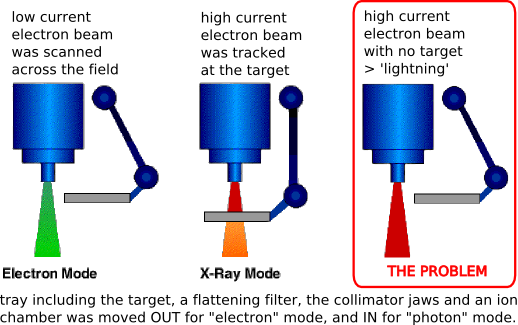
\includegraphics[width=2.5in]{../img/Therac25.png}
		\label{fig:knight}
	\end{figure}



\end{frame}
%%%%%%%%%%%%%%%%%%%%%%%%%%%%%%%%%%%%%%%%%%%%%%%%%%%%%%%%%%%%%%%%%%%%%%%%%%%%%%%%%%%%%%%%%%%%%%%%%%%%%%%%%
\begin{frame}{Falhas são Caras}
	
	\begin{itemize}
		\item Manter ou desenvolver novas funcionalidades é bem mais caro que o custo de criação\cite{tan2005comparing}.
	\end{itemize}


	\begin{figure}[!t]
		\centering
		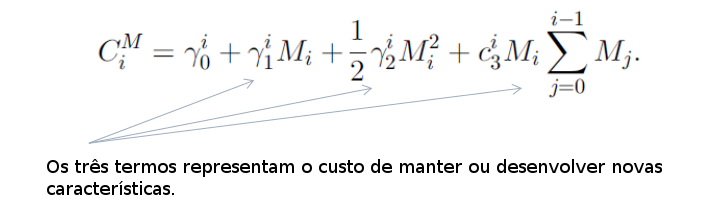
\includegraphics[width=4.5in]{../img/custo_manutencao.png}
		\label{fig:knight}
	\end{figure}
	
\end{frame}

%%%%%%%%%%%%%%%%%%%%%%%%%%%%%%%%%%%%%%%%%%%%%%%%%%%%%%%%%%%%%%%%%%%%%%%%%%%%%%%%%%%%%%%%%%%%%%%%%%%%%%%%%%
\begin{frame}{Falhas podem dormir}
	
	\begin{itemize}
		\item Um erro pode levar algum tempo até se manifestar
	\end{itemize}


	\begin{figure}[!t]
		\centering
		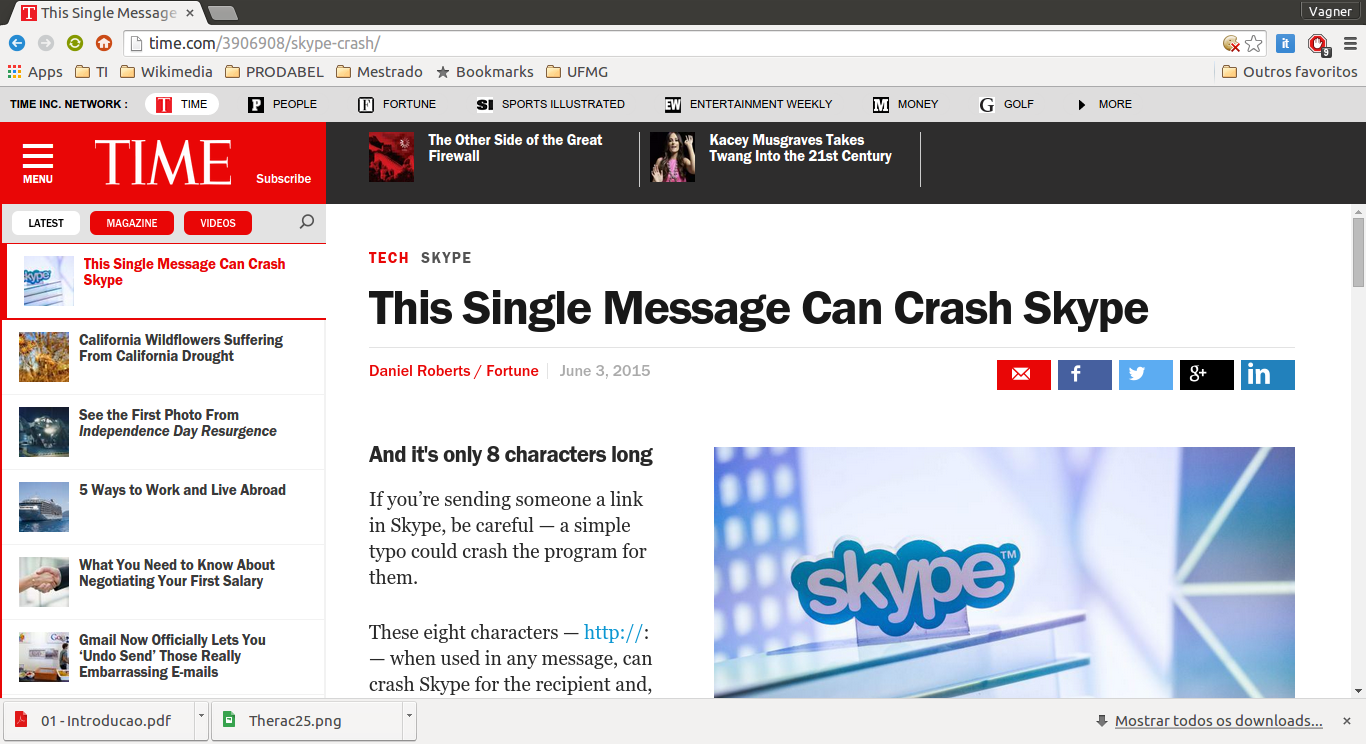
\includegraphics[width=4.5in]{../img/erro_skype.png}
		\label{fig:knight}
	\end{figure}
\end{frame}

%%%%%%%%%%%%%%%%%%%%%%%%%%%%%%%%%%%%%%%%%%%%%%%%%%%%%%%%%%%%%%%%%%%%%%%%%%%%%%%%%%%%%%%%%%%%%%%%%%%%%%%%%%
\begin{frame}{Confiabilidade de Software}

	\begin{itemize}
		\item Conforme a ANSI é definida como a probabilidade de operação de um produto de software livre de falhas por um período de tempo em um ambiente.
		\item Possibilidade de classificar os módulos de um sistema a partir de sua \alert{Confiabilidade}
		\item \alert{Problema:} Baseado no tempo de execução do software.
	\end{itemize}


\end{frame}
%%%%%%%%%%%%%%%%%%%%%%%%%%%%%%%%%%%%%%%%%%%%%%%%%%%%%%%%%%%%%%%%%%%%%%%%%%%%%%%%%%%%%%%%%%%%%%%%%%%%%%%%%%%%
\begin{frame}{Confiabilidade em Hardware}

	\begin{figure}[!t]
		\centering
		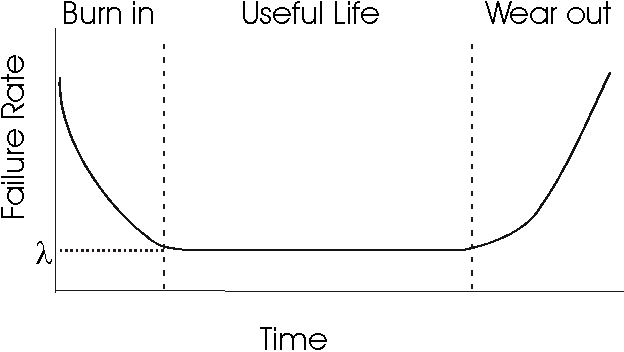
\includegraphics[width=3.5in]{../img/bath_curve.png}
		\label{fig:bath_curve}
		\caption{Curva Bathtub para a Confiabilidade de Hardware. Adaptado de \cite{Lyu:1996}}
	\end{figure}


\end{frame}

%%%%%%%%%%%%%%%%%%%%%%%%%%%%%%%%%%%%%%%%%%%%%%%%%%%%%%%%%%%%%%%%%%%%%%%%%%%%%%%%%%%%%%%%%%%%%%%%%%%%%%%%%%%

\begin{frame}{Confiabilidade em Software}

	\begin{figure}[!t]
		\centering
		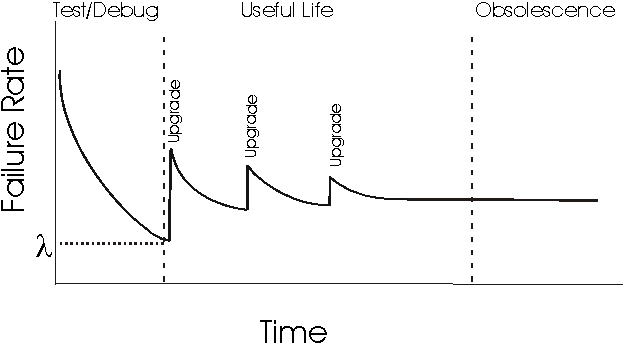
\includegraphics[width=3.5in]{../img/bath_curve_sw.png}
		\label{fig:bath_curve}
		\caption{Curva Bathtub para a Confiabilidade de Software. Adaptado de \cite{Lyu:1996}}
	\end{figure}


\end{frame}
%%%%%%%%%%%%%%%%%%%%%%%%%%%%%%%%%%%%%%%%%%%%%%%%%%%%%%%%%%%%%%%%%%%%%%%%%%%%%%%%%%%%%%%%%%%%%%%%%%%%%%

\begin{frame}{Métricas de Software}

	\begin{itemize}
		
		\item Utilizadas com o objetivo de mensurar a qualidade interna do software.
		\item Baseadas em Thresholds
		\item Fortemente dependente do paradigma e linguagem utilizada no sistema avaliado.	
	\end{itemize}


\end{frame}
%%%%%%%%%%%%%%%%%%%%%%%%%%%%%%%%%%%%%%%%%%%%%%%%%%%%%%%%%%%%%%%%%%%%%%%%%%%%%%%%%%%%%%%%%%%%%55
\section{Problema}
\begin{frame}{Problemas}

	\begin{itemize}
		\item Modelos de Confiabilidade são dependentes do tempo de execução.
		\item Métricas de Software são baseadas em threshold.
		\item Inexistência de um \alert{Modelo de Predição da Confiabilidade} que considere valores das \alert{Métricas de Software}
	\end{itemize}

\end{frame}
%%%%%%%%%%%%%%%%%%%%%%%%%%%%%%%%%%%%%%%%%%%%%%%%%%%%%%%%%%%%%%%%%%%%%%%%%%%%%%%%%%%%%%%%%%%%%%%%%%%%
\section{Objetivo}
\begin{frame}{Objetivo}

	\begin{itemize}
		\item Propor \alert{Modelo de Predição da Confiabilidade} que vise definir os módulos com o maior número de falhas utilizando \alert{dados históricos} e \alert{Métricas de Software}.
	\end{itemize}

\end{frame}
%%%%%%%%%%%%%%%%%%%%%%%%%%%%%%%%%%%%%%%%%%%%%%%%%%%%%%%%%%%%%%%%%%%%%%%%%%%%%%%%%%%%%%%%%%%%%%%%%%%%%%%%
\section{Modelo Proposto}
\begin{frame}{Modelo Proposto}
	\begin{itemize}
		\item Seja $X_{vc}=[X_1,X_2,\ldots,X_k]$ um vetor de característica de uma versão $v$ de
um componente $c$ de um determinado sistema.
		\item  Seja ainda $\lambda$ a taxa média de falhas do componente $c$.
		\item Podemos definir uma função de característica $\varphi_{vc}$ conforme Equação \ref{eq:fun_carac}{}.
	\end{itemize}
	\begin{equation} \label{eq:fun_carac}
    		\varphi_{vc} = \sum_{j=1}^{k} \frac{1}{w_{j}} \times X_{jc}
	\end{equation}

\end{frame}
%%%%%%%%%%%%%%%%%%%%%%%%%%%%%%%%%%%%%%%%%%%%%%%%%%%%%%%%%%%%%%%%%%%%%%%%%%%%%%%%%%%%%%%%%%%%%%%%%%%%%%%%%
\begin{frame}{Modelo Proposto}

	\begin{itemize}
		\item Na Equação \ref{eq:fun_carac} o valor de $k$ representa o tamanho do conjunto de
métricas;
		\item $w{j}$ refere-se ao peso da métrica no cálculo da função de característica;
		\item  $X_{jc}$ é o valor da métrica $X_j$ obtida do componente $c$.
		
	\end{itemize}
	
\end{frame}
%%%%%%%%%%%%%%%%%%%%%%%%%%%%%%%%%%%%%%%%%%%%%%%%%%%%%%%%%%%%%%%%%%%%%%%%%%%%%%%%%%%%%%%%%%%%%%%%%%%%%%%%%%%55

\begin{frame}{Modelo Proposto}

	\begin{itemize}
		\item A partir de $\varphi_{vc}$ é possível calcular o número de erros em determinado módulo com base na Equação \ref{eq:fun_erros}{}.
	\end{itemize}
	
	\begin{equation} \label{eq:fun_erros}
    		\omega = \lambda \times \frac{\varphi_{vc}}{\varphi_{(v-1)c}}
	\end{equation}
\end{frame}
%%%%%%%%%%%%%%%%%%%%%%%%%%%%%%%%%%%%%%%%%%%%%%%%%%%%%%%%%%%%%%%%%%%%%%%%%%%%%%%%%%%%%%%%%%%%%%%%%%%%%%%%%%%55
\begin{frame}{Conjunto de Métricas}
	
	\begin{itemize}
		\item Neste trabalho foi utilizado a suite \alert{CK-Metrics} \cite{chidamber1994metrics}
		\item Conjunto de Métricas largamente utilizado na literatura.
		\item Capaz detectar classes mais propensas a falhas \cite{basili1996validation}
	\end{itemize}

\end{frame}

%%%%%%%%%%%%%%%%%%%%%%%%%%%%%%%%%%%%%%%%%%%%%%%%%%%%%%%%%%%%%%%%%%%%%%%%%%%%%%%%%%%%%%%%%%%%%%%%%%%%%%%%%%%
\begin{frame}{CK-Metrics}
	
	\begin{itemize}
	\item \textit{Weighted Methods per Class (WMC)} 
	\item \textit{Depth of Inheritance Tree (DIT)}
	\item \textit{Number Of Children(NOC)}
	\item \textit{Coupling Between Objects(CBO)}	
	\item \textit{Response For a Class (RFC)}	
	\item \textit{Lack of Cohesion on Methods (LCOM)}
	\end{itemize}

\end{frame}

%%%%%%%%%%%%%%%%%%%%%%%%%%%%%%%%%%%%%%%%%%%%%%%%%%%%%%%%%%%%%%%%%%%%%%%%%%%%%%%%%%%%%%%%%%%%%%%%%%%%%%%%%%%%%
\section{Avaliação}

\begin{frame}{Avaliação do Modelo}
	\begin{itemize}
		\item Coletado os dados de bugs de quatro sistemas implementados em Java
		\item Desenvolvidos pela Apache Software Foundation\footnote{\url{http://www.apache.org}}
		\item Critério de escolha:
		\begin{itemize}
			\item Base de usuários abrangente e ativa.
			\item Um grande número de bugs registrados no BST da Apache Foundation
			\item Pertencente a diferentes categorias de software.
		\end{itemize}
	\end{itemize}

\end{frame}

%%%%%%%%%%%%%%%%%%%%%%%%%%%%%%%%%%%%%%%%%%%%%%%%%%%%%%%%%%%%%%%%%%%%%%%%%%%%%%%%%%%%%%%%%%%%%%%%%%%%%%%%%%%%%

\begin{frame}{Sistemas Utilizados}

\begin{table}[h]
\resizebox{\textwidth}{!}{%
\begin{tabular}{|l|l|l|c|}
\hline
\multicolumn{1}{|c|}{{\bf Produto}} & \multicolumn{1}{c|}{{\bf Descrição}} & \multicolumn{1}{c|}{{\bf Categoria}} & {\bf KLOC} \\ \hline
\textit{Ant} & Ferramenta utilizada para automação de compilação de software. & Gerenciamento da Compilação & 133\\ \hline
\textit{JMeter} & Ferramenta utilizada para testes de carga em um servidores, redes ou objetos Java. & Ferramenta de Testes & 92 \\ \hline
\textit{Log4j} & API para que o desenvolvedor de software possa fazer log de dados na aplicação. & Biblioteca & 15 \\ \hline
\textit{Tomcat 7} & Servidor web Java que implementa as tecnologias Java Servlet e JavaServer Pages. & Servidor Web & 196 \\ \hline
\end{tabular}
}
\caption{Sistemas utilizados na avaliação}
\label{tab:sistemas}
\end{table}
\end{frame}
%%%%%%%%%%%%%%%%%%%%%%%%%%%%%%%%%%%%%%%%%%%%%%%%%%%%%%%%%%%%%%%%%%%%%%%%%%%%%%%%%%%%%%%%%%%%%%%%%%%%%%%%

\begin{frame}{Dados Coletados}

\begin{table}[h]
\resizebox{\textwidth}{!}{%
\begin{tabular}{|l|l|}
\hline
\multicolumn{1}{|c|}{{\bf Campo}} & \multicolumn{1}{c|}{{\bf Descrição}}                                                             \\ \hline
\textit{ID}                                & Identificador de um bug no ASF Bugzilla                                                          \\ \hline
Situação                          		  & Identifica o estado atual de um bug.                                                             \\ \hline
\textit{Produto}                           & O sistema no qual o bug ocorreu                                                                  \\ \hline
\textit{Versão}                            & A versão do sistema em que o bug ocorreu                                                         \\ \hline
\textit{Componente}                        & Identifica o módulo do sistema em que o bug ocorreu                                              \\ \hline
\textit{Hardware}                          & A plataforma de hardware no qual o erro foi observado.                                           \\ \hline
\textit{Importância}                       & A importância de um bug é descrita como a combinação de sua prioridade e gravidade.              \\ \hline
\textit{Target Milestone}                  & O campo   Target Milestone identifica em qual versão do sistema o bug deverá estar selecionado. \\ \hline
\textit{Atribuído Para}                    & Identifica o responsável pela resolução do bug.                                                   \\ \hline
\textit{Data do Bug}                       & Contêm a data em que o bug foi reportado.                                 \\ \hline
\textit{Relatado Por}                      & Identifica o responsável por informar o bug.                                                      \\ \hline
\textit{Data da Ultima Alteração}          & Contêm a data da última alteração ocorrida na resolução do bug. \\ \hline
\textit{Descrição do Bug}                  & Contêm os detalhes do problema reportado.                                                         \\ \hline
\end{tabular}
}
\caption{Campos recuperados pelo \textit{ASFBugScraper}\footnote{Sistema criado para realizar um scraping na página do ASF Bugzilla}}
\label{tab:campos}
\end{table}
\end{frame}
%%%%%%%%%%%%%%%%%%%%%%%%%%%%%%%%%%%%%%%%%%%%%%%%%%%%%%%%%%%%%%%%%%%%%%%%%%%%%%%%%%%%%%%%%%%%%%%%%%%%%

\begin{frame}{Seleção dos Dados}
	\begin{itemize}
		\item Considerados apenas os bugs confirmados
		\item Os bugs foi divididos em duas categorias \textsc{CAT-HIST} e \textsc{CAT-LAST}.
		\begin{itemize}
			\item \textsc{CAT-HIST} - Bugs em versões diferente da última avaliada.
			\item \textsc{CAT-LAST} - Bugs da última versão do sistema analisada.
		\end{itemize}
		\item Falhas em \textsc{CAT-HIST} foram utilizados para de calcular a taxa de confiabilidade $\omega$ 			\item Os valores de $\omega$ são comparados com os bugs em \textsc{CAT-LAST}.
	\end{itemize}
\end{frame}

%%%%%%%%%%%%%%%%%%%%%%%%%%%%%%%%%%%%%%%%%%%%%%%%%%%%%%%%%%%%%%%%%%%%%%%%%%%%%%%%%%%%%%%%%%%%%%%%%%%%%%%

\begin{frame}{Categorização das versões dos sistemas}


\begin{table}[htbp]
\resizebox{\textwidth}{!}{%
\begin{tabular}{|c|c|c||c|c|c|}
\hline
\textbf{Sistema} & \textbf{Versões em CAT-HIST} & \textbf{Tamanho da Amostra} & \textbf{Versão em CAT-LAST} & \textbf{Tamanho da Amostra} & \textbf{Total Bugs}\\
\hline

\multirow{2}{*}{\textit{Ant}} 	 & 1.0; 1.1; 1.2; 1.3; 1.4.x & & & &\\
							 	 & 1.5.x; 1.6.x; 1.7.x; 1.8.x & 3097 & 1.9.5 & 98 & \textbf{3195}\\
\hline

\multirow{2}{*}{\textit{JMeter}}  & 1.5; 1.7.x; 1.8.x; 1.9.x; 2.0.x & & & &\\
								 & 2.1.x; 2.2.x; 2.3.x; 2.4.x; 2.5.x; 2.6; 2.7; 2.8 & 1415 & 2.9 & 140 & 												\textbf{1555}\\
\hline
								 
\textit{Log4j} & 1.0; 1.1 & 224 & 1.2.18 & 539 & \textbf{763}\\
\hline
\multirow{10}{*}{\textit{Tomcat 7}} & 7.0.0; 7.0.1; 7.0.2; 7.0.3; 7.0.4; 7.0.5; & & & & \\
								 & 7.0.6; 7.0.7; 7.0.8; 7.0.9; 7.0.10; 7.0.11; & & & & \\
								 & 7.0.12; 7.0.13; 7.0.14; 7.0.15; 7.0.16; 7.0.17; & & & & \\
								 & 7.0.18; 7.0.19; 7.0.20; 7.0.21; 7.0.22; 7.0.23; & & & &  \\
								 & 7.0.24; 7.0.25; 7.0.26; 7.0.27;7.0.28;7.0.29;& 475 & 7.0.59 & 11 & \textbf{486}\\
								 & 7.0.30; 7.0.31; 7.0.32; 7.0.33; 7.0.34; 7.0.35; & & & & \\
								 & 7.0.36; 7.0.37; 7.0.38; 7.0.39; 7.0.40; 7.0.41; & & & & \\
								 & 7.0.42; 7.0.43; 7.0.44; 7.0.45; 7.0.46; 7.0.47; & & & & \\
								 & 7.0.48; 7.0.49; 7.0.50; 7.0.51; 7.0.52; 7.0.53; & & & & \\
								 & 7.0.54; 7.0.55; 7.0.56; 7.0.57 & & & & \\
\hline
\end{tabular}
}
\caption{Categorização das versões dos sistemas}
\label{tab:categorias}
\end{table}

\end{frame}
%%%%%%%%%%%%%%%%%%%%%%%%%%%%%%%%%%%%%%%%%%%%%%%%%%%%%%%%%%%%%%%%%%%%%%%%%%%%%%%%%%%%%%%%%%%%%%%%%%%%%%%%%5
\begin{frame}{Coletando as Métricas}

	\begin{itemize}
		\item Métricas coletadas utilizando a ferramenta \textit{ckjm}\cite{Jur10}
		\item Código compilado dos sistemas recuperados diretamente do site da Apache Foundation
		\item Métricas por classe vs Falhas por ``módulo"
		\begin{itemize}
			\item Distinção dos módulos pelo nome dos packages
			\item Considerado a média das métricas das classes como o valor de um módulo.
		\end{itemize}
	\end{itemize}


\end{frame}
%%%%%%%%%%%%%%%%%%%%%%%%%%%%%%%%%%%%%%%%%%%%%%%%%%%%%%%%%%%%%%%%%%%%%%%%%%%%%%%%%%%%%%%%%%%%%%%%%%%%%%%%
\section{Resultados}

\begin{frame}{Resultados}

\begin{table}[h]
\centering
\resizebox{\textwidth}{!}{%
\begin{tabular}{|l|l|c|l|l|l|l|l|l|l|l|c|c|}
\hline
\multicolumn{1}{|c|}{{\bf Sistema}}        & \multicolumn{1}{c|}{{\bf Componente}} & {\bf Taxa Média de Falhas} & \multicolumn{1}{c|}{{\bf Versão}} & \multicolumn{1}{c|}{{\bf WMC}} & \multicolumn{1}{c|}{{\bf DIT}} & \multicolumn{1}{c|}{{\bf NOC}} & \multicolumn{1}{c|}{{\bf CBO}} & \multicolumn{1}{c|}{{\bf RFC}} & \multicolumn{1}{c|}{{\bf LCOM}} & \multicolumn{1}{c|}{{\bf $\varphi_{vc}$}} & {\bf $\frac{\varphi_{vc}}{\varphi_{(v-1)c}}$}    & {\bf $\omega$}                 \\ \hline
\multicolumn{1}{|c|}{\multirow{6}{*}{Ant}} & \multirow{2}{*}{Core}                 & \multirow{2}{*}{16,96}     & 1.9.4                             & 8,705                          & 0,521                          & 0,421                          & 7,687                          & 26,515                         & 63,983                          & 107,831                         & \multirow{2}{*}{1,027} & \multirow{2}{*}{17,420} \\ \cline{4-11}
\multicolumn{1}{|c|}{}                     &                                       &                            & 1.9.3                             & 8,695                          & 0,503                          & 0,435                          & 7,691                          & 26,423                         & 61,240                          & 104,985                         &                        &                         \\ \cline{2-13} 
\multicolumn{1}{|c|}{}                     & \multirow{2}{*}{Core tasks}           & \multirow{2}{*}{42,87}     & 1.9.4                             & 9,710                          & 0,914                          & 0,247                          & 6,720                          & 27,043                         & 166,968                         & 211,602                         & \multirow{2}{*}{1,007} & \multirow{2}{*}{43,177} \\ \cline{4-11}
\multicolumn{1}{|c|}{}                     &                                       &                            & 1.9.3                             & 9,688                          & 0,914                          & 0,247                          & 6,720                          & 26,989                         & 165,538                         & 210,097                         &                        &                         \\ \cline{2-13} 
\multicolumn{1}{|c|}{}                     & \multirow{2}{*}{Optional Tasks}       & \multirow{2}{*}{20,18}     & 1.9.4                             & 11,311                         & 1,410                          & 0,049                          & 4,492                          & 25,754                         & 87,852                          & 130,869                         & \multirow{2}{*}{1,000} & \multirow{2}{*}{20,180} \\ \cline{4-11}
\multicolumn{1}{|c|}{}                     &                                       &                            & 1.9.3                             & 11,311                         & 1,410                          & 0,049                          & 4,492                          & 25,754                         & 87,852                          & 130,869                         &                        &                         \\ \hline
\multirow{4}{*}{Jmeter}                    & \multirow{2}{*}{Main}                 & \multirow{2}{*}{12,29}     & 2.9                               & 8,769                          & 0,929                          & 0,380                          & 8,196                          & 21,757                         & 101,673                         & 141,704                         & \multirow{2}{*}{0,981} & \multirow{2}{*}{12,055} \\ \cline{4-11}
                                           &                                       &                            & 2.8                               & 8,900                          & 0,949                          & 0,377                          & 8,383                          & 22,057                         & 103,801                         & 144,467                         &                        &                         \\ \cline{2-13} 
                                           & \multirow{2}{*}{HTTP}                 & \multirow{2}{*}{26,23}     & 2.9                               & 7,793                          & 0,868                          & 0,245                          & 9,199                          & 22,852                         & 53,926                          & 94,883                          & \multirow{2}{*}{1,015} & \multirow{2}{*}{26,618} \\ \cline{4-11}
                                           &                                       &                            & 2.8                               & 7,691                          & 0,866                          & 0,246                          & 9,188                          & 22,567                         & 52,942                          & 93,501                          &                        &                         \\ \hline
\multirow{4}{*}{Log4j}                     & \multirow{2}{*}{Configurator}         & \multirow{2}{*}{13,14}     & 1.2.17                            & 7,308                          & 1,000                          & 0,000                          & 8,077                          & 28,154                         & 56,308                          & 100,846                         & \multirow{2}{*}{1,115} & \multirow{2}{*}{14,654} \\ \cline{4-11}
                                           &                                       &                            & 1.2.16                            & 6,500                          & 1,000                          & 0,000                          & 8,357                          & 25,714                         & 48,857                          & 90,429                          &                        &                         \\ \cline{2-13} 
                                           & \multirow{2}{*}{Appender}             & \multirow{2}{*}{44}        & 1.2.17                            & 10,967                         & 0,600                          & 0,533                          & 6,667                          & 30,367                         & 38,800                          & 87,933                          & \multirow{2}{*}{0,976} & \multirow{2}{*}{42,957} \\ \cline{4-11}
                                           &                                       &                            & 1.2.16                            & 10,862                         & 0,621                          & 0,517                          & 7,172                          & 30,069                         & 40,828                          & 90,069                          &                        &                         \\ \hline
\multirow{2}{*}{Tomcat}                    & \multirow{2}{*}{Catalina}             & \multirow{2}{*}{7,42}      & 7.0.59                            & 9,121                          & 0,121                          & 0,788                          & 3,455                          & 22,152                         & 54,727                          & 90,364                          & \multirow{2}{*}{0,947} & \multirow{2}{*}{7,027}  \\ \cline{4-11}
                                           &                                       &                            & 7.0.57                            & 9,581                          & 0,129                          & 0,774                          & 3,484                          & 23,258                         & 58,194                          & 95,419                          &                        &                         \\ \hline
\end{tabular}
}
\caption{CK Métricas e o valor de w}
\label{tab:ck_metricas}
\end{table}

	


\end{frame}
%%%%%%%%%%%%%%%%%%%%%%%%%%%%%%%%%%%%%%%%%%%%%%%%%%%%%%%%%%%%%%%%%%%%%%%%%%%%%%%%%%%%%%%%%%%%%%%%%%%%%%%%

\begin{frame}{Resultados}

	
\begin{table}[h]
\centering
\resizebox{\textwidth}{!}{%
\begin{tabular}{|l|l|c|c|c|c|c|}
\hline
\multicolumn{1}{|c|}{{\bf Sistema}} & \multicolumn{1}{c|}{{\bf Componente}} & {\bf Média} & {\bf Total Erros} & {\bf Erros Encontrados(\%)} & {\bf $\omega$} & {\bf Erros Previstos (\%)} \\ \hline
Ant                                 & Core                                  & 16,96       & 7                 & 23,33\%                     & 17,42   & 21,57\%                    \\ \hline
Ant                                 & Core tasks                            & 42,87       & 20                & 66,67\%                     & 43,177  & 53,45\%                    \\ \hline
Ant                                 & Optional Tasks                        & 20,18       & 3                 & 10,00\%                     & 20,18   & 24,98\%                    \\ \hline
Jmeter                              & HTTP                                  & 12,29       & 27                & 19,29\%                     & 12,055  & 31,17\%                    \\ \hline
Jmeter                              & Main                                  & 26,23       & 113               & 80,71\%                     & 26,618  & 68,83\%                    \\ \hline
Log4j                               & Appender                              & 13,14       & 7                 & 87,50\%                     & 14,654  & 25,44\%                    \\ \hline
Log4j                               & Configurator                          & 44          & 1                 & 12,50\%                     & 42,957  & 74,56\%                    \\ \hline
Tomcat 7                            & Catalina                              & 7,42        & 6                 & -                           & 7,027   & -                          \\ \hline
\end{tabular}
}
\caption{Valores Coletados x Valores Previstos}
\label{tab:res_relativo}
\end{table}


\end{frame}
%%%%%%%%%%%%%%%%%%%%%%%%%%%%%%%%%%%%%%%%%%%%%%%%%%%%%%%%%%%%%%%%%%%%%%%%%%%%%%%%%%%%%%%%%%%%%%%%%%%%%%%%


\begin{frame}{Resultados - Ant}

\begin{figure}[htbp]
\centering
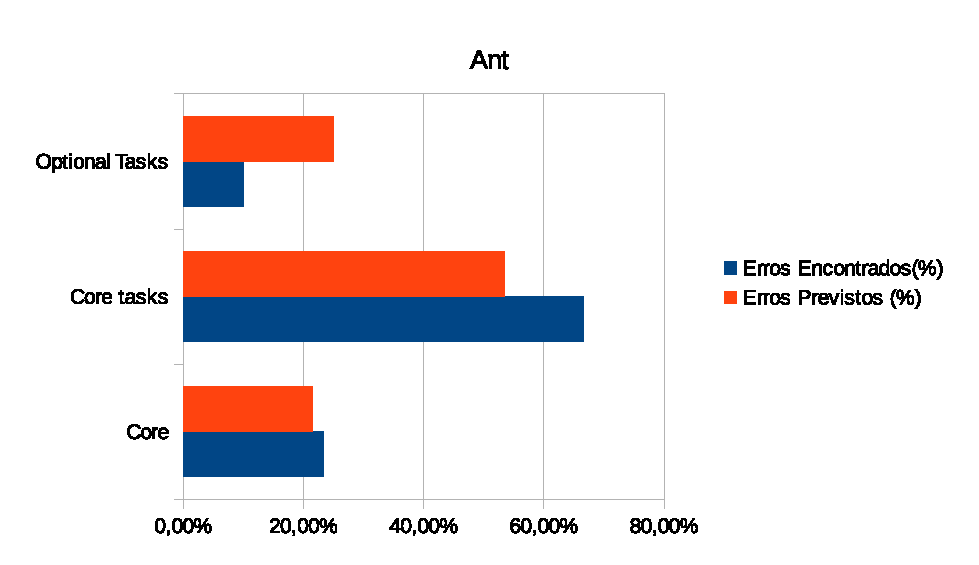
\includegraphics[width=.80\textwidth]{../img/graph_ant.eps}
\caption{Resultados Sistema Ant}
\label{fig:avalicao_ant}
\end{figure}	


\end{frame}
%%%%%%%%%%%%%%%%%%%%%%%%%%%%%%%%%%%%%%%%%%%%%%%%%%%%%%%%%%%%%%%%%%%%%%%%%%%%%%%%%%%%%%%%%%%%%%%%%%%%%%%%


\begin{frame}{Resultados-JMeter}

\begin{figure}[htbp]
\centering
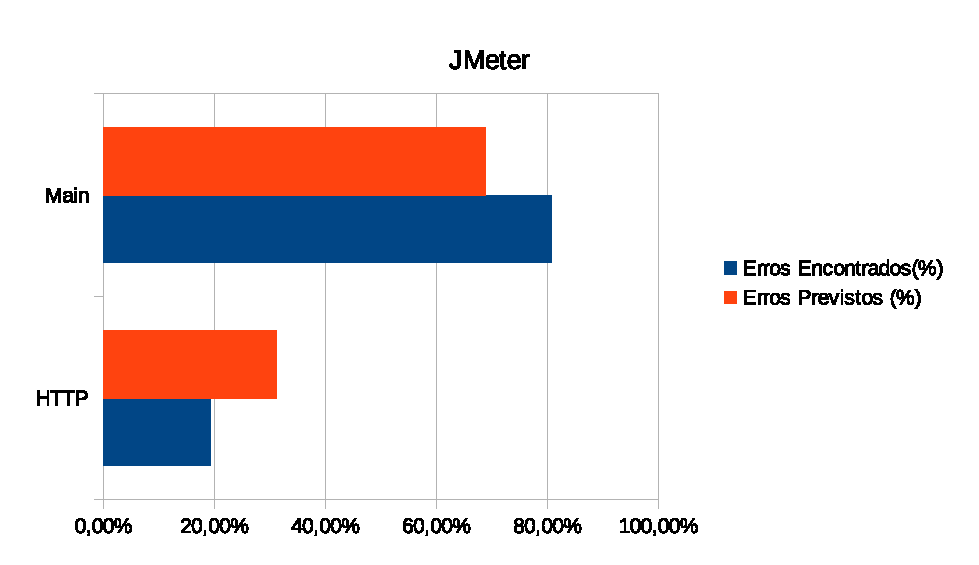
\includegraphics[width=.80\textwidth]{../img/graph_jmeter.eps}
\caption{Resultados Sistema JMeter}
\label{fig:avalicao_jmeter}
\end{figure}
	


\end{frame}
%%%%%%%%%%%%%%%%%%%%%%%%%%%%%%%%%%%%%%%%%%%%%%%%%%%%%%%%%%%%%%%%%%%%%%%%%%%%%%%%%%%%%%%%%%%%%%%%%%%%%%%%



\begin{frame}{Resultados-Log4J}

\begin{figure}[htbp]
\centering
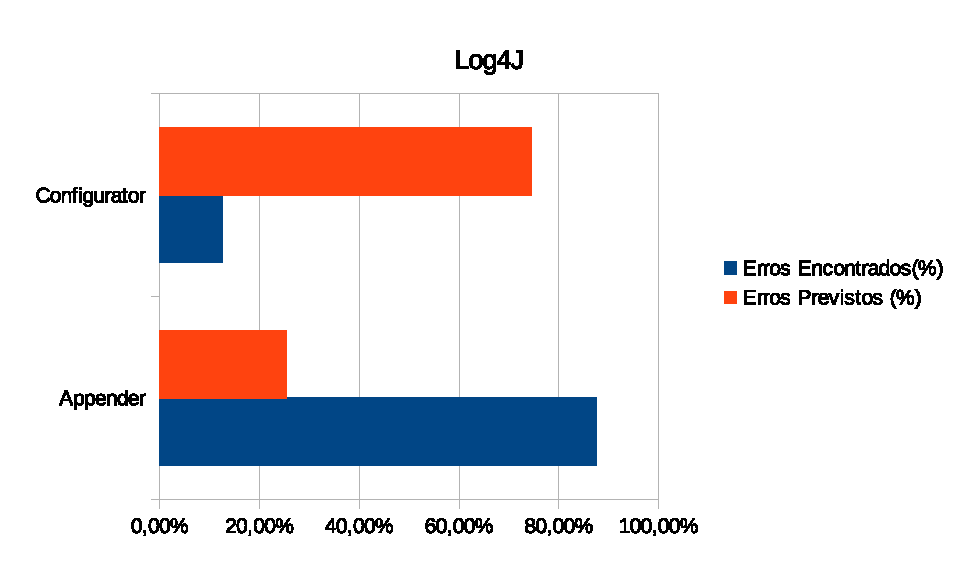
\includegraphics[width=.80\textwidth]{../img/graph_log4j.eps}
\caption{Resultados Sistema Log4J}
\label{fig:avalicao_log4j}
\end{figure}


\end{frame}
%%%%%%%%%%%%%%%%%%%%%%%%%%%%%%%%%%%%%%%%%%%%%%%%%%%%%%%%%%%%%%%%%%%%%%%%%%%%%%%%%%%%%%%%%%%%%%%%%%%%%%%%
\section{Trabalhos Relacionados}

\begin{frame}{Trabalhos Relacionados}
	\begin{itemize}
	
		\item Em \textit{Chidamber et al.}\cite{chidamber1994metrics} é proposto um conjunto de métricas para a análise de sistemas orientados a objeto.
		\item No trabalho de \textit{Basili et. al.} \cite{basili1996validation} as métricas proposta por \cite{chidamber1994metrics} foram utilizadas para buscar classes mais propensas a falhas.
	\end{itemize}

\end{frame}

\begin{frame}{Trabalhos Relacionados}
	\begin{itemize}
	\item Em \textit{Eaddy et al.} \cite{eaddy2008crosscutting} é discutido o efeito de Crosscutting Concerns nas falhas dos sistemas com base em dados recuperados de um repositório de software.		
	\item Em \textit{Salem et al.}\cite{salem2004prediction} foi utilizado a técnica de regressão logística com o objetivo de predizer falhas.	
	\end{itemize}

\end{frame}


\section{Ameaças à Validade}
\begin{frame}{Ameaças à Validade}

	\begin{itemize}
	
		\item Medição da taxa de Confiabilidade em uma granularidade ao nível de módulo.
		\item Utilização da média das métricas.
		\item Número de sistemas avaliados bem como a linguagem utilizada.
		\item Os sistemas foram desenvolvidos pela mesma organização.
		\item As falhas foram ``aceitas" por diferentes desenvolvedores.
	\end{itemize}		
	
\end{frame}

\section{Conclusões e Trabalhos Futuros}
\begin{frame}{Trabalhos Futuros}
	
	\begin{itemize}
		\item Este trabalho demostra a importância do uso de métricas de software na análise da qualidade interna do produto de software.
		\item O uso de dados históricos junto com métricas de software podem aumentar a qualidade dos modelos de predição de falhas.
	\end{itemize}

\end{frame}


\begin{frame}{Trabalhos Futuros}
	\begin{itemize}
	
		\item Refinar o modelo visando uma melhor predição.
		\item Coletar maiores informações para testar o modelo ao nível de classe.
		\item Aplicar o modelo em softwares de outras linguagens e organizações.

	\end{itemize}

\end{frame}

\begin{frame}{Dúvidas}

\begin{figure}[htbp]
\centering

\includegraphics[width=.80\textwidth]{../img/questions.jpg}
\label{fig:questoes}
\end{figure}	

\end{frame}

\begin{frame}[allowframebreaks]
   \frametitle{References}
   \bibliographystyle{IEEEtranS}
   \bibliography{IEEEfull,bibliografia}
\end{frame}

\end{document}
